\section{Results}

% As above, clarity, correctness, and suitability of the presentation, discussion, and conclusions
% that you draw are the major grading criteria. Other aspects, such as
% presentation style, relevance of the text (everything that is needed,
% but no irrelevant and unnecessary information), etc. apply as well.

To account for participants' typing speed difference, each individual participant's WPM was normalized to their average WPM across all tests.

Participants' average WPM, accuracy and comfort level were plotted against the visual latency in milliseconds, as well as the sample index of the test. The plots are shown in Figure~\ref{fig:results}.

\begin{figure}[h]
    \centering
    
    \begin{subfigure}[b]{1.0\linewidth}
        \centering
        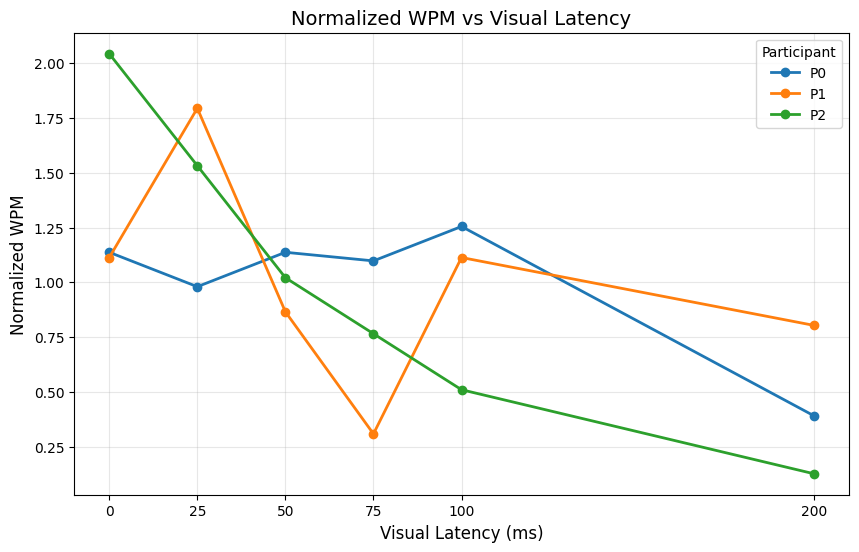
\includegraphics[width=\linewidth]{resources/nwpm-vs-latency.png}
        \caption{Normalized WPM vs. latency.}
        \label{fig:setup}
    \end{subfigure}
    
    \vspace{1em}
    
    \begin{subfigure}[b]{1.0\linewidth}
        \centering
        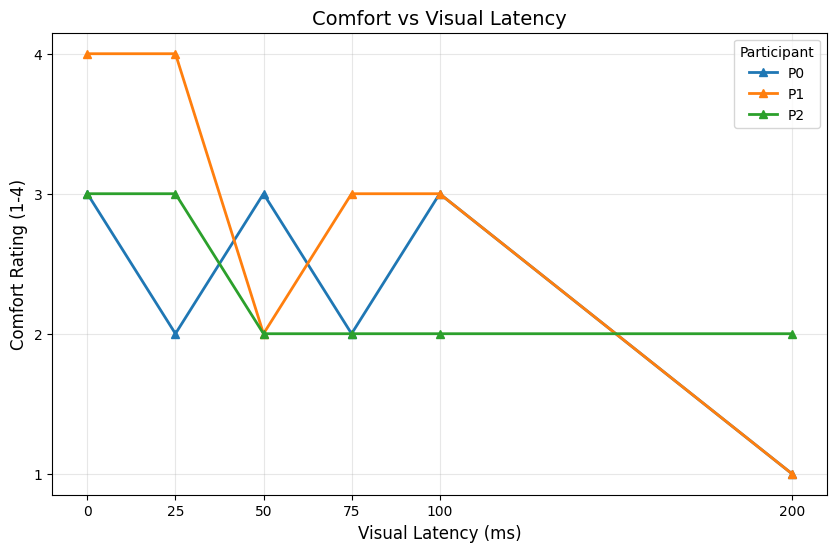
\includegraphics[width=\linewidth]{resources/comfort-vs-latency.png}
        \caption{Perceived comfort level vs. latency.}
        \label{fig:comfort}
    \end{subfigure}
    
    \caption{Participants' normalized words-per-minute (WPM) and perceived comfort level plotted against latency.}
    \label{fig:results}
\end{figure}


